\documentclass{article}
\usepackage{graphicx} % Required for inserting images
\usepackage{german}
\usepackage{amsmath}
\usepackage{amssymb}
\usepackage{amsthm}
\usepackage{url}
\usepackage{tikz}
\usetikzlibrary{arrows.meta}




\newcommand{\R}{\mathbb{R}}% reele Zahlen
\newcommand{\C}{\mathbb{C}}% komplexe Zahlen
\newcommand{\Q}{\mathbb{Q}}% rationale Zahlen


\newtheorem{thm}{Satz}
\newtheorem{cor}[thm]{Korollar}
\newtheorem{lem}[thm]{Lemma}
\newtheorem{prop}[thm]{Proposition}
\newtheorem{defn}[thm]{Definiton}


\title{Sortieralgorithmen}
\date{\today}
\author{Maya Neudorf\\ \url{maya.neudorf@uni-bielefeld.de}}
\newpage
\begin{document}

\newpage
\maketitle
\tableofcontents
\newpage
\section{Was ist eine Ordnung?}
Diese Ausarbeitung befasst sich mit Sortieralgorithmen. Um zu sortieren führen wir erst einmal den Begriff einer Ordnung ein. 
\begin{defn}
 Sei $S$ eine Menge. Eine Relation $R \subseteq S \times S$ heißt partielle Ordnung $\preceq$, wenn folgende Eigenschaften gelten:
    \begin{itemize}
        \item[(a)] $(a,a) \in R$  (Reflexität);
        \item[(b)]$((a,b) \in R \wedge (b,a) \in R) \Rightarrow a=b$  (Antisymmetrie)
	\item [(c)]$((a,b \in R \wedge (b,c) \in R \Rightarrow (a,c) \in R$  (Transitivität)
    \end{itemize}
\end{defn}
Die Teilmengen Relation $\subseteq$ ist ein Beispiel für so eine partielle Ordnung.
\begin{defn}
 Eine partielle Ordnung R von S heißt totale Ordnung, wenn $(a,b) \in R$ oder $(b,a) \in R$ für alle $a,b \in S$ gilt 
\end{defn}
Beispiel für eine totale Ordnung ist die gewohnte Ordnung $\le$ auf          $\mathbb{R}$.

\section{das allgemeine Sortierproblem}

Um eine Liste zu sortieren suchen wir einen Algorithmus der mit folgender Eingabe und Ausgabe arbeitet:
\begin{itemize}
\item \textbf{Input:}
eine endliche Menge $S$ mit einer partiellen Ordnung $\preceq$
\\
\item \textbf{Output:}
Berechne eine Bijektion $f \colon \{1,\dots,n\} \to S$ mit $f(j) \not\preceq f(i)$ für alle $1\le i<j \le n$ (eine sortierte Liste)
\end{itemize}
Die naive Herangehensweise wäre einfach die $n!$ Permutaionen auszuprobieren und jeweils zu testen ob die Liste geordnet ist. Dies istnatürlich sehr ineffizient.

\section{Sortieren durch sukzessive Auswahl}



\begin{itemize}
\item \textbf{Input:} eine Menge $S = \{s_1, \dots, s_n\}$; eine partielle Ordnung $\preceq $ auf $S$ 
\item \textbf{Output:}  eine Bijektion $f: \{1, \dots, n\} \to S$ mit $f(j) \not\preceq f(i)$ für alle $1 \le i < j \le n$.
\end{itemize}
\textbf{for}{$i \leftarrow 1$ \textbf{to} $n$} \textbf{do} $f(i) \leftarrow s_i$\\
    \textbf{for}{$i \leftarrow 1$ \textbf{to} $n$}\\
        \textbf{for}{$j \leftarrow i$ \textbf{to} $n$}\\
            \textbf{if}{$f(j) \le f(i)$} 
                \textbf{then swap}($f(i), f(j)$)\\
            \textbf{output} $f$


Praktisch würde der Algorithmus bei der Liste {3,4,2,1} also wiefolgt vorgehen. Beim ersten Durchlauf, also $i=1$, vergleicht der Algorithmus alle Elemente der Liste und findet so das kleinste. Dieses kleinste Element in der Liste, also die 1, wird nach ganz vorne geschrieben. Nach einer Iteration sieht die Liste also so aus:{1,3,4,2}. Nun bei $i=2$ wird die 2 herausgesucht und hinter die eins geschrieben ({1,2,3,4}).Obwohl wir als Menschen genau sehen, dass die Liste nun geordnet ist, muss der Algorithmus noch die zwei Iterationen durchführen. Der Algorithmus vergleicht also viermal alle vier Zahlen miteinander.

\textbf{Die Laufzeit beträgt also $O(n^2)$.}

\subsection{Beweis für Korrektheit des Algorithmus}

Intuitiv ist sehr schnell klar, dass dieser Algorithmus funktioniert. Trotzdem wird dies im folgenden formell bewiesen.
Wir zeigen, dass für alle $1 \le i \le j \le n$  nach Iteration (i,j) folgendes gilt:
\begin{itemize}
\item[(a)]$f(k) \not \preceq f(i) $ für alle $1 \le h <i$ und $h<k\le n$ (vor i ist die Liste sortiert)
\item[(b)]$f(k) \not \preceq f(i)$ für alle $i<k \le j$ (i ist kleiner als alles rechts davon)
\end{itemize}
% eventuell itemizen
Für b)  1.Fall $f(j)\not \preceq f(i)$: es wird nichts getauscht. b) gilt also
	2.Fall:$ f(j) \preceq f(i)$, betrachte Index $k$ mit $i<k \le j$: für $j=k$ gilt wegen der Antisymmetrie b) nach dem swap-Befehl.
für $k<j$ galt zuvor $f(k)\not\preceq f(i)$ und somit $f(k) \not\preceq f(j)$. Es gilt also b).

\section{Sortieren nach Schlüsseln}

Für schnellere Sortieralgorithmen benötigen wir ein totale Ordnung. Um diese zu erzwingen definieren wir eine Abbildung $k:S\rightarrow K$ von der Menge der zu sortierenden Elemente S zu einer Menge von Schlüsseln K mt einer totalen Ordnung.
\begin{itemize}\item\textbf{Input:}eine endliche Menge $S$, sowie eine Funktion $k:S\rightarrow K$ und eine totale Ordnung $\le$ auf K.
\item\textbf{Output:}
Berechne eine Bijektion $f \colon \{1,\dots,n\} \to S$ mit $k(f(j)) \not\le k(f(i))$ für alle $1\le i<j \le n$ (eine sortierte Liste von Schlüsseln)
\end{itemize}
\textbf{Beispiele:}
Bucketsort, Insertion sort, Bubblesort

\subsection{Bubblesort}

Bei Bubblesort wird die Liste (n-1)-mal durchgegeanen und die Elemente werden jeweils verglichen. Wenn ein Element gefunden wird, dass kleiner als sein Vorgänger ist, werden Vorgänger und das Element vertauscht.
Bubblesort würde die Liste (3,2,4,1) also wie folgt sotieren:\\
1.Iteration: (2,3,1,4) \\
2.Iteration: (2,1,3,4)\\
3.Iteration: (1,2,3,4)\\
Diese Verfahren ist also manchmal schneller, braucht aber für manche Instanzen trotzdem viele Vergleiche.

\section{Mergesort}

\begin{itemize}\item \textbf{Input:}
eine  Menge $S=\{s_1; \cdots ;s_n \}$; eine durch Schlüssel induzierte partielle Ordnung $\preceq$ auf $S$.\item\textbf{Output:}
Berechne eine Bijektion $f \colon \{1,\dots,n\} \to S$ mit $f(j) \not\preceq f(i)$ für alle $1\le i<j \le n$.
 \end{itemize}
 

\textbf{if}$|S| > 1$ \\
\textbf{then} \begin{itemize}
 \item sei $S = S_1 \; \dot{\cup}\;S_2$ mit $|S_1| = \lfloor \frac{n}{2} \rfloor$ und $|S_2| =\lceil \frac{n}{2} \rceil$
\item sortiere $S_1$ und $S_2$(rekursiv mit Mergesort)
\item  Verschmelze die Sortierungen von $S_1$ und $S_2$ zu Sortierung $S$.

\end{itemize}
Mergesort beruht also auf dem „Divide-and-Conquer“-Prinzip. Man teilet das Ausgangsproblem in kleinere Teilprobleme, löst diese separat, und füge die Listen geordnet wieder zusammen.

\subsection{Laufzeit}
Mergesort sortiert $n$ Elemente in der Laufzeit $O(n log n)$
 \\
 \textbf{Beweis:}
Sei $c \in \mathbb{N}$ mit $T(1) \leq c$ und 
\[
T(n) \leq T(\lfloor \tfrac{n}{2} \rfloor) + T(\lceil \tfrac{n}{2} \rceil) + cn \quad \text{für alle } n \geq 2.
\]

\textbf{Behauptung:} $T(2^k) \leq c(k+1)2^k$ für alle $k \in \mathbb{N} \cup \{0\}$.

Induktion über $k$: 
Für $k = 0$ trivial. 

Für $k \in \mathbb{N}$ gilt:
$T(2^k) \leq 2 \cdot T(2^{k-1}) + c 2^k \leq 2 \cdot ck 2^{k-1} + c 2^k = c(k+1)2^k.$

$\Rightarrow   n \in \mathbb{N}$ mit $k := \lceil \log_2 n \rceil < 1 + \log_2 n$:

$T(n) \leq T(2^k) \leq c(k+1)2^k < 2c(2 + \log_2 n)n = O(n \log n).$

\subsection{Satz zur Anzahl von Vergleichen}
\begin{thm}
Jeder Sortieralgorithmus, der nur mit paarweisen Vergleichen von zwei Elementen arbeitet, benötigt zum sortieren einer n-elementigen Menge mindestens $log_2(n!)$ Vergleiche.
\end{thm}
Der Beweis dieses Satzes lässt sich mit folgendem beispielhaften Vergleichsbaum für n=3 veranschaulichen: \\

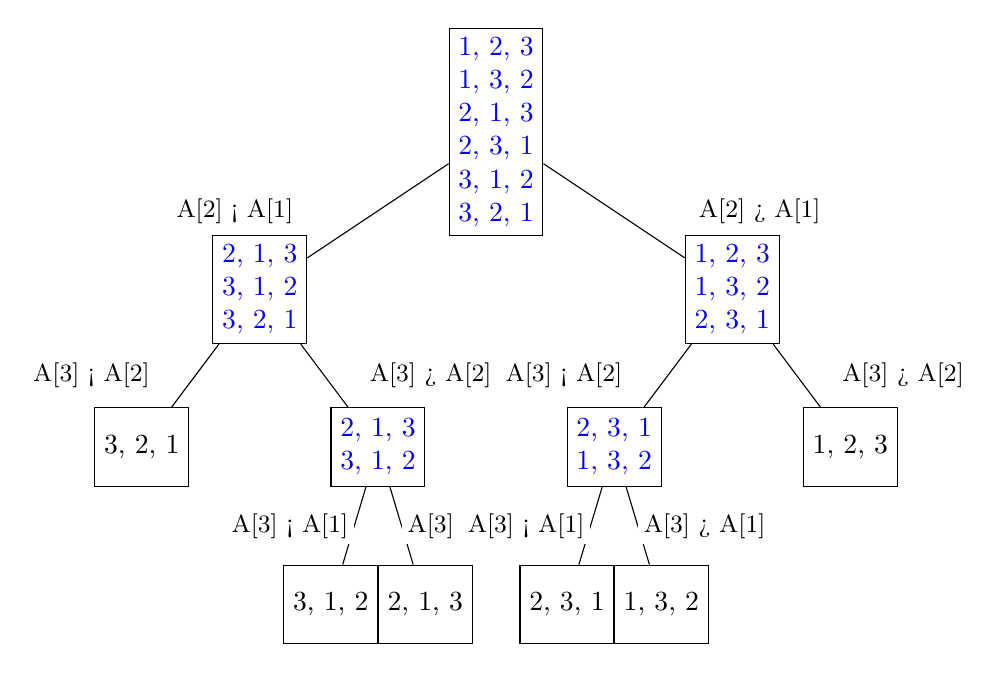
\begin{tikzpicture}[
    level distance=2cm,
    level 1/.style={sibling distance=6cm},
    level 2/.style={sibling distance=3cm},
    level 3/.style={sibling distance=1.2cm},
    box/.style={draw, rectangle, align=center, minimum height=1cm, color=blue},
    edge_label/.style={fill=white, font=\small, inner sep=2pt}
]

% Wurzelknoten
\node[box, black] (root) {\color{blue} 1, 2, 3 \\ \color{blue} 1, 3, 2 \\ \color{blue} 2, 1, 3 \\ \color{blue} 2, 3, 1 \\ \color{blue} 3, 1, 2 \\ \color{blue} 3, 2, 1}
    child {
        node[box, black] (n1) {\color{blue} 2, 1, 3 \\ \color{blue} 3, 1, 2 \\ \color{blue} 3, 2, 1}
        child {
            node[box, black] {3, 2, 1}
            edge from parent node[edge_label, left, xshift=-0.5cm] {A[3] < A[2]}
        }
        child {
            node[box, black] (n12) {\color{blue} 2, 1, 3 \\ \color{blue} 3, 1, 2}
            child {
                node[box, black] {3, 1, 2}
                edge from parent node[edge_label, left] {A[3] < A[1]}
            }
            child {
                node[box, black] {2, 1, 3}
                edge from parent node[edge_label, right] {A[3] > A[1]}
            }
            edge from parent node[edge_label, right, xshift=0.5cm] {A[3] > A[2]}
        }
        edge from parent node[edge_label, left, xshift=-1cm] {A[2] < A[1]}
    }
    child {
        node[box, black] (n2) {\color{blue} 1, 2, 3 \\ \color{blue} 1, 3, 2 \\ \color{blue} 2, 3, 1}
        child {
            node[box, black] (n21) {\color{blue} 2, 3, 1 \\ \color{blue} 1, 3, 2}
            child {
                node[box, black] {2, 3, 1}
                edge from parent node[edge_label, left] {A[3] < A[1]}
            }
            child {
                node[box, black] {1, 3, 2}
                edge from parent node[edge_label, right] {A[3] > A[1]}
            }
            edge from parent node[edge_label, left, xshift=-0.5cm] {A[3] < A[2]}
        }
        child {
            node[box, black] {1, 2, 3}
            edge from parent node[edge_label, right, xshift=0.5cm] {A[3] > A[2]}
        }
        edge from parent node[edge_label, right, xshift=1cm] {A[2] > A[1]}
    };

\end{tikzpicture}
\\

\textbf{Beweis:}
Gegeben: Eingabemenge $S=\{1,\cdots,n\}$ mit einer totalen Ordnung

Gesucht: einer der n! Permutationen (Blätter im Vergleichsbaum). 
Jeder Vergleich halbiert die Anzahl an möglichen Permtationen (ein Vergleich ist ein Schritt im Baum).
Ein Algorithmus braucht also $k$ Vergleiche mit $2^k\ge n! $$\Rightarrow k\ge \log_2(n!)$.

Im Allgemeinen werden mehr Vegleiche gebraucht. Beispielweise werden für n=5 7 Vergleiche gebraucht und nicht $\log_2(5!)=6.9$ Vergleiche.

\section{Quicksort}
Im folgendem betrachten wir eine abgewandelte Form des mergesort.

\begin{itemize}\item\textbf{Input}
eine  Menge $S=\{s_1; \cdots ;s_n \}$; eine durch Schlüssel induzierte partielle Ordnung $\preceq$ auf $S$.\item \textbf{Output}
Berechne eine Bijektion $f \colon \{1,\dots,n\} \to S$ mit $f(j) \not\le f(i)$ für alle $1\le i<j \le n$.


\textbf{if}{$|S| > 1$} \\
\textbf{then} \begin{itemize} \item wähle $x\in S$ beliebig
     \item $S_1 := \{s \in S \mid s \leq x\} \setminus \{x\}$
    \item$S_2 := \{s \in S \mid x \leq s\} \setminus \{x\}$
   \item $S_x := S \setminus (S_1 \cup S_2)$
    \item Sortiere $S_1$ und $S_2$ (soweit nicht leer) rekursiv mit Quicksort
    \item  Füge die sortierten Mengen $S_1$, $S_x$ und $S_2$ aneinander
    \end{itemize}
 \end{itemize}
 Ein Vorteil bei Quicksort ist, dass kein zusätzlicher temporärer Speicherplatz benötigt wird.
 \subsection{Laufzeit}
 Quicksort sortiert $n$ Elemente in der Laufzeit $O(n^2)$.\\
 \textbf{Beweis:}
 Es exististiert ein $c\in \mathbb{N}$ mit $T(1) \leq c$.
$T(n)\leq cn + \max_{\substack{0\leq l \leq n-1}}(T(l)+T(n-1-l))
 $ für alle $n\geq 2$.\\
 Behauptung:$T(n)\leq cn^2 $\\
 Beweis per Induktion über n: Für $n=1$ trivial.\\
 $T(n)\leq \max_{\substack{0\leq l \leq n-1}}(cl^2+c(n-1-l)^2) = cn+ c(n-1)^2 < cn^2$
 \subsection{die Wahl des x}
 Beim Quicksort macht es einen großen Unterschied wie das x gewählt wird. Für kleine Listen oder schon relativ sortierte Listen macht es Sinn immer das erste Element der Liste als x zu wählen. %erkläore 
 Dann haben wir die oben bewiesene Laufzeit. Alternativ kann auch durch einen Zufallsalgorithmus ein zufälliges Element als x gewählt werden. Das scheint zwar erste einmal effektiver beläuft sich aber auf die selbe worst-case Laufzeit.
 Eine andere Möglchkeit wäre erst einmal den Median zu ermitteln und ihn als x zu wählen. Der Median kann in einer Zeit von $O(n)$ ermittelt werden und die Laufzeit würde sich dadurch auf $O(n logn) $ verkürzen. Bei besonders großen Listen macht dies zwar manchmal Sinn, lohnt sich generell aber selten.  
\subsection{Erwartungswert} {Der Erwartungswert der Laufzeit von Random-Quicksort für $n$ Elemente ist $O(n log(n))$}.
\\ \textbf{Beweis:}
Es exististiert ein $c\in \mathbb{N}$ mit $\overline{T}(1) \leq c$.
$\overline{T}(n)\leq cn + \frac{1}{n} \sum_{i=1}^{n} (\overline{T}(i-1) + \overline{T}(n-i)) = cn + \frac{2}{n} \sum_{i=1}^{n-1} \overline{T}(i)
 $ für alle $n\geq 2$.\\
 \textbf{Behauptung:} $\overline{T}(n) < 2cn(1 + \ln n)$. \\
Wir zeigen dies per Induktion über $n$. Für $n = 1$ ist die Aussage trivial. Für $n \geq 2$ erhalten wir mit der Induktionsvoraussetzung:

\begin{align*}
\overline{T}(n) &\leq cn + \frac{2}{n} \sum_{i=1}^{n-1} 2ci(1 + \ln i) \\
&\leq cn + \frac{2c}{n} \int_{1}^{n} 2x(1 + \ln x) \, dx \\
&= cn + \frac{2c}{n} \left[ x^2(1 + \ln x) - \frac{x^2}{2} \right]_{1}^{n} \\
&= cn + 2cn(1 + \ln n) - cn - \frac{c}{n} < 2cn(1 + \ln n)
\end{align*}
Diese exzellente Laufzeit macht den Random-Quicksort relativ attraktiv.

\section{Heapsort}

\begin{defn}
 Ein \textbf{Heap} für eine endliche Menge $S$ mit Schlüsseln $k: S \to K$ und einer totalen Ordnung $\leq$ von $K$ ist eine Arboreszenz (ein gerichteter Graph) $A$ mit einer Bijektion $f: V(A) \to S$, so dass die Heapordnung
 
$k(f(v)) \leq k(f(w)) \quad \text{für alle } (v, w) \in E(A) $
gilt.(Ein Baum, in dem jedes Elternteil einen kleineren Wert hat als seine Kinder)
\end{defn}
Der Algorithmus, der so einen Heap erstellt arbeitet wie folgt:
Beim Einfügen eines Elements in einen Heap mit bislang n Elementen wird dieses zunächst
dem Knoten n zugeordnet. Anschließend wird das Element mit seinem Vogänger verglichen und vertauscht solange bis der Vorgänger größer ist. \\ Beim Löschen eines Elements aus einem Heap mit n Elementen wird zunächst das nte Element an die Stelle des gelöschten Elements gesetzt und dann werden verschiedene Funktionen angewandt um die Heapordnung wiederherzustellen. 


Beispiel fülr das Einfügen eines Elements: \\
 \\
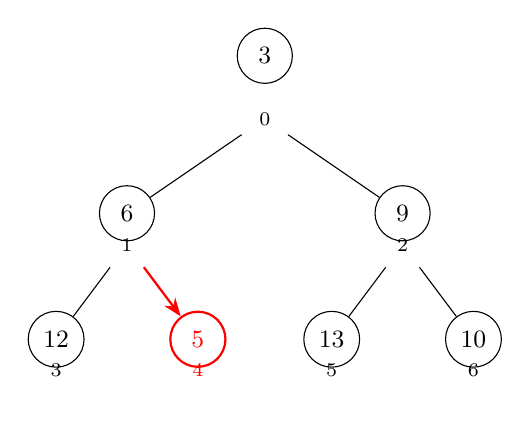
\begin{tikzpicture}[
    every node/.style={circle, draw, minimum size=0.7cm, font=\small},
    level distance=1.2cm,
    level 1/.style={sibling distance=3.5cm},
    level 2/.style={sibling distance=1.8cm},
    level 3/.style={sibling distance=1.0cm},
    idx/.style={draw=none, font=\scriptsize, yshift=-0.4cm} % Style für die Index-Zahlen
]

\node {3} [idx] node[idx] {0}
    child {node {6} node[idx] {1}
        child {node {12} node[idx] {3}}
        child {node[red, thick] {5} node[idx, red] {4} edge from parent[red, thick, -{Stealth}]}
        }
    child {node {9} node[idx] {2}
        child {node {13} node[idx] {5}}
        child {node {10} node[idx] {6}}
    };

\end{tikzpicture}
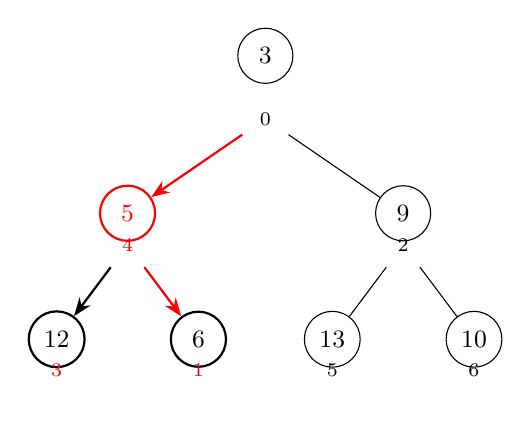
\begin{tikzpicture}[
    every node/.style={circle, draw, minimum size=0.7cm, font=\small},
    level distance=1.2cm,
    level 1/.style={sibling distance=3.5cm},
    level 2/.style={sibling distance=1.8cm},
    level 3/.style={sibling distance=1.0cm},
    idx/.style={draw=none, font=\scriptsize, yshift=-0.4cm} % Style für die Index-Zahlen
]

\node {3} [idx] node[idx] {0}
    child {node[red, thick] {5} node[idx, red] {4} edge from parent[red, thick, -{Stealth}]
        child {node [black, thick]{12} node[idx] {3}edge from parent[black, thick]}
        child {node [black, thick]{6} node[idx] {1}}
        }
    child {node {9} node[idx] {2}
        child {node {13} node[idx] {5}}
        child {node {10} node[idx] {6}}
    };

\end{tikzpicture}

\end{document}







